% This file was created with tikzplotlib v0.10.1.
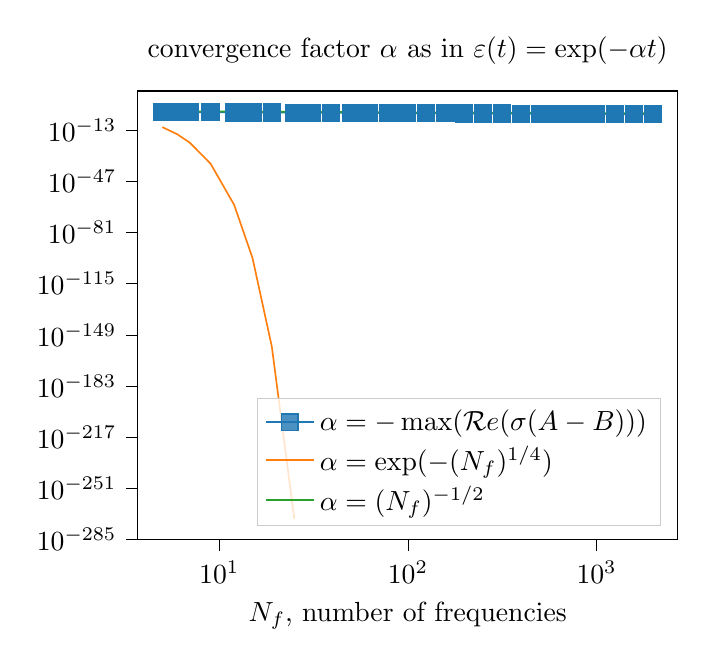
\begin{tikzpicture}

\definecolor{darkgray176}{RGB}{176,176,176}
\definecolor{darkorange25512714}{RGB}{255,127,14}
\definecolor{forestgreen4416044}{RGB}{44,160,44}
\definecolor{lightgray204}{RGB}{204,204,204}
\definecolor{steelblue31119180}{RGB}{31,119,180}

\begin{axis}[
legend cell align={left},
legend style={
  fill opacity=0.8,
  draw opacity=1,
  text opacity=1,
  at={(0.97,0.03)},
  anchor=south east,
  draw=lightgray204
},
log basis x={10},
log basis y={10},
tick align=outside,
tick pos=left,
title={convergence factor $\alpha$ as in $\varepsilon(t) = \exp(-\alpha t)$},
x grid style={darkgray176},
xlabel={$N_f$, number of frequencies},
xmin=3.70660110378415, xmax=2684.39999919113,
xminorgrids,
xmode=log,
xtick style={color=black},
xtick={0.1,1,10,100,1000,10000,100000},
xticklabels={
  $\mathdefault{10^{-1}}$,
  $\mathdefault{10^{0}}$,
  $\mathdefault{10^{1}}$,
  $\mathdefault{10^{2}}$,
  $\mathdefault{10^{3}}$,
  $\mathdefault{10^{4}}$,
  $\mathdefault{10^{5}}$
},
y grid style={darkgray176},
ymin=1.02735491052278e-285, ymax=16022980612467.1,
yminorgrids,
ymode=log,
ytick style={color=black},
ytick={9.99988867182683e-320,1e-285,1e-251,1e-217,1e-183,1e-149,1e-115,1e-81,1e-47,1e-13,1e+21,1e+55},
yticklabels={
  ,
  $\mathdefault{10^{-285}}$,
  $\mathdefault{10^{-251}}$,
  $\mathdefault{10^{-217}}$,
  $\mathdefault{10^{-183}}$,
  $\mathdefault{10^{-149}}$,
  $\mathdefault{10^{-115}}$,
  $\mathdefault{10^{-81}}$,
  $\mathdefault{10^{-47}}$,
  $\mathdefault{10^{-13}}$,
  $\mathdefault{10^{21}}$,
  $\mathdefault{10^{55}}$
}
]
\addplot [semithick, steelblue31119180, mark=square*, mark size=3, mark options={solid}]
table {%
5 0.115617739171503
6 0.108646928336916
7 0.103356447022984
9 0.0949483578418249
12 0.0856284794601421
15 0.0785271304178387
19 0.0711014898412081
25 0.0590317377319682
31 0.0512704592800944
39 0.0444147273709822
50 0.0382508943085019
62 0.0337343140486478
79 0.0293699535618058
99 0.0258677218998984
125 0.0227190783387875
158 0.0199601504403576
199 0.0175799373602619
250 0.0155087111397549
315 0.013659570500855
398 0.012011267054205
500 0.010593261488627
629 0.00933378243442911
792 0.00821843697078803
997 0.00723568966791155
1255 0.00634930074273194
1581 0.0055752846645051
1990 0.00490290047452506
};
\addlegendentry{$\alpha = -\max(\mathcal{R}e(\sigma(A-B)))$}
\addplot [semithick, darkorange25512714]
table {%
5 1.3887943864964e-11
6 2.31952283024357e-16
7 5.24288566336346e-22
9 6.63967719958073e-36
12 2.8946403116483e-63
15 1.92194772782385e-98
19 1.65841047768115e-157
25 3.6808558548018e-272
31 0
39 0
50 0
62 0
79 0
99 0
125 0
158 0
199 0
250 0
315 0
398 0
500 0
629 0
792 0
997 0
1255 0
1581 0
1990 0
};
\addlegendentry{$\alpha = \exp(-(N_f)^{1/4})$}
\addplot [semithick, forestgreen4416044]
table {%
5 0.447213595499958
6 0.408248290463863
7 0.377964473009227
9 0.333333333333333
12 0.288675134594813
15 0.258198889747161
19 0.229415733870562
25 0.2
31 0.179605302026775
39 0.160128153805087
50 0.14142135623731
62 0.127000127000191
79 0.112508790092602
99 0.100503781525921
125 0.0894427190999916
158 0.079555728417573
199 0.0708881205008336
250 0.0632455532033676
315 0.0563436169819011
398 0.0501254707117086
500 0.0447213595499958
629 0.039872611141445
792 0.0355334527259351
997 0.0316703177609768
1255 0.0282278718468818
1581 0.0251497727413928
1990 0.022416791983111
};
\addlegendentry{$\alpha = (N_f)^{-1/2}$}
\end{axis}

\end{tikzpicture}
